% !TEX root = ../TAMU_Thesis_Main.tex

%%%%%%%%%%%%%%%%%%%%%%%%%%%%%%%%%%%%%%%%%%%%%%%%%%%%%%%%%%%%%%%%%%%%%%
%%                           SECTION IV
%%%%%%%%%%%%%%%%%%%%%%%%%%%%%%%%%%%%%%%%%%%%%%%%%%%%%%%%%%%%%%%%%%%%%

\chapter{SUMMARY AND CONCLUSIONS \label{cha:Summary}}

The summary goes here, along with your conclusions. The title of this final chapter/section must contain the words ``summary'' or ``conclusions.''

Here, I attempt to fill the section with more figures, possibly more tables. The inclusion of these floats is to manipulate the list of figures and list of tables in order to see when the inconsistent spacing begins. It is important to remember that any images you wish to use are placed in the appropriate directory inside the folder in which the project is kept. In the original template, all the images used as figures here are placed in the subdirectory \textit{graphics}, as declared in the preamble of \textit{TAMUTemplate.tex}. If you wish to use any other directories, be sure to declare them in the preamble of \textit{TAMUTemplate.tex}. See the figure below on how to declare directories.

\begin{figure}[h!]
	\centering
	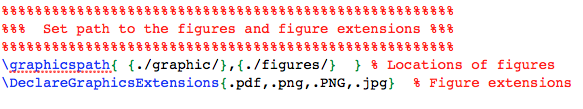
\includegraphics[scale=0.95]{GraphicDir.png}
	\caption{Declaring graphics directories.}
\end{figure}

This version of the template now has a section to place any packages that you are using - see the figure below.

\begin{figure}[!h]
	\centering
	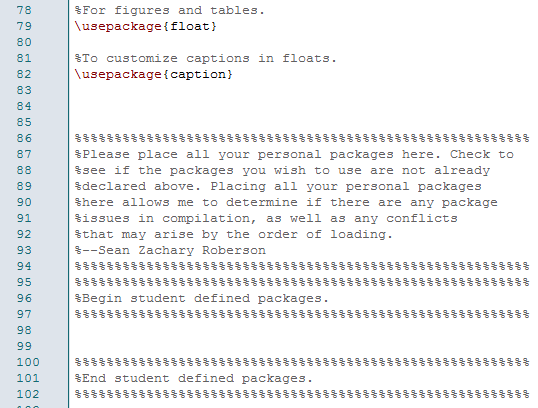
\includegraphics[scale=0.95]{CustomPackage.png}
	\caption{The place to declare any packages you require that I have not already declared. This simplifies debugging.}
\end{figure}

More figures will be inserted, with some text between them.

\begin{figure}[!h]
	\centering
	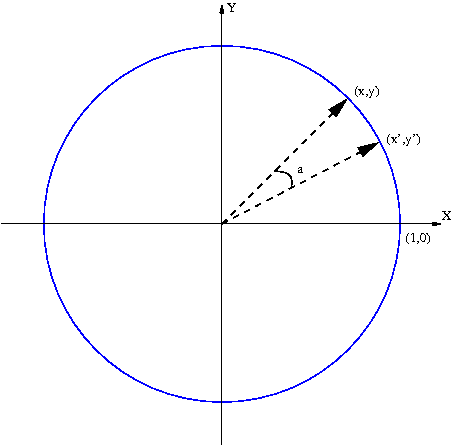
\includegraphics[scale=0.85]{CartesianCoordinate.png}
	\caption{Two points on the unit circle and their corresponding position vectors.}
\end{figure}

This section has filler text. These words serve no meaning except to fill a few lines in the document. This section has filler text. These words serve no meaning except to fill a few lines in the document. This section has filler text. These words serve no meaning except to fill a few lines in the document. This section has filler text. These words serve no meaning except to fill a few lines in the document. This section has filler text. These words serve no meaning except to fill a few lines in the document. This section has filler text. These words serve no meaning except to fill a few lines in the document. This section has filler text. These words serve no meaning except to fill a few lines in the document. This section has filler text. These words serve no meaning except to fill a few lines in the document. This section has filler text. These words serve no meaning except to fill a few lines in the document. This section has filler text. These words serve no meaning except to fill a few lines in the document. This section has filler text. These words serve no meaning except to fill a few lines in the document. This section has filler text. These words serve no meaning except to fill a few lines in the document.

\begin{figure}[!h]
	\centering
	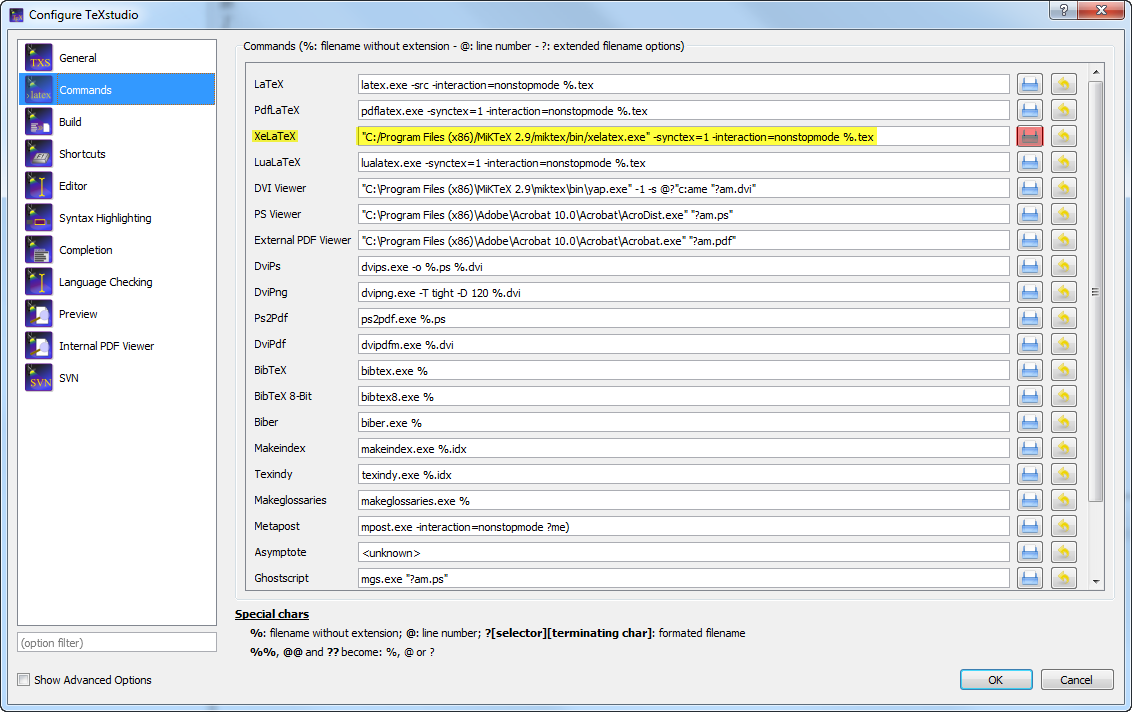
\includegraphics[width=4.25in]{CompileChange.png}
	\caption{Changing the method of compilation for XeLaTeX in TeXstudio.}
\end{figure}

This section has filler text. These words serve no meaning except to fill a few lines in the document. This section has filler text. These words serve no meaning except to fill a few lines in the document. This section has filler text. These words serve no meaning except to fill a few lines in the document. This section has filler text. These words serve no meaning except to fill a few lines in the document. This section has filler text. These words serve no meaning except to fill a few lines in the document. This section has filler text. These words serve no meaning except to fill a few lines in the document. This section has filler text. These words serve no meaning except to fill a few lines in the document. This section has filler text. These words serve no meaning except to fill a few lines in the document. This section has filler text. These words serve no meaning except to fill a few lines in the document. This section has filler text. These words serve no meaning except to fill a few lines in the document. This section has filler text. These words serve no meaning except to fill a few lines in the document. This section has filler text. These words serve no meaning except to fill a few lines in the document. This section has filler text. These words serve no meaning except to fill a few lines in the document. This section has filler text. These words serve no meaning except to fill a few lines in the document. This section has filler text. These words serve no meaning except to fill a few lines in the document. This section has filler text. These words serve no meaning except to fill a few lines in the document. This section has filler text. These words serve no meaning except to fill a few lines in the document. This section has filler text. These words serve no meaning except to fill a few lines in the document.

\begin{figure}[!h]
	\centering
	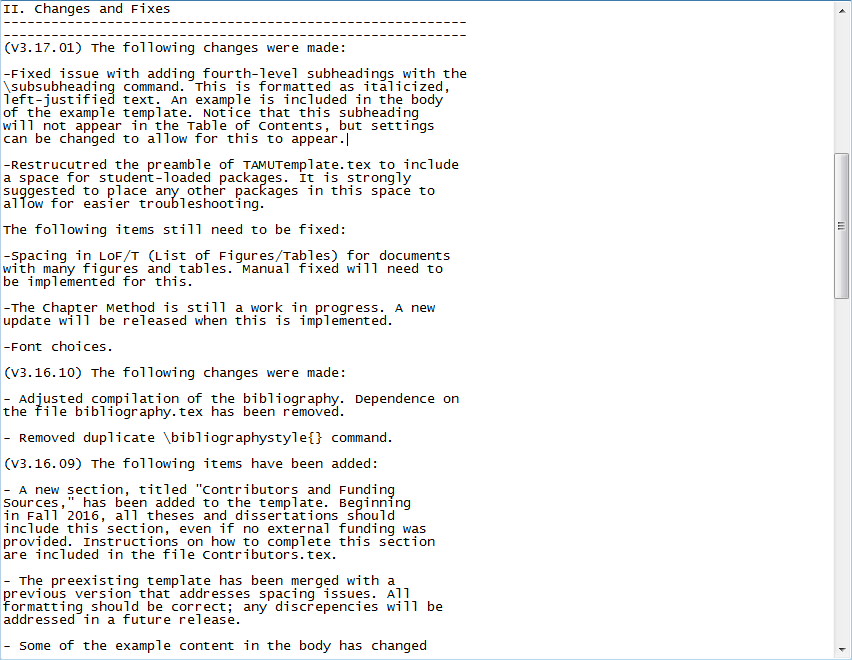
\includegraphics[width = 4.825in]{Changelog.png}
	\caption{A portion of the changelog in the README for this document. This is located in the root directory.}
\end{figure}

This section has filler text. These words serve no meaning except to fill a few lines in the document. This section has filler text. These words serve no meaning except to fill a few lines in the document. This section has filler text. These words serve no meaning except to fill a few lines in the document. This section has filler text. These words serve no meaning except to fill a few lines in the document. This section has filler text. These words serve no meaning except to fill a few lines in the document. This section has filler text. These words serve no meaning except to fill a few lines in the document.

This section has filler text. These words serve no meaning except to fill a few lines in the document. This section has filler text. These words serve no meaning except to fill a few lines in the document. This section has filler text. These words serve no meaning except to fill a few lines in the document. This section has filler text. These words serve no meaning except to fill a few lines in the document. This section has filler text. These words serve no meaning except to fill a few lines in the document. This section has filler text. These words serve no meaning except to fill a few lines in the document. This section has filler text. These words serve no meaning except to fill a few lines in the document. This section has filler text. These words serve no meaning except to fill a few lines in the document. This section has filler text. These words serve no meaning except to fill a few lines in the document. This section has filler text. These words serve no meaning except to fill a few lines in the document. This section has filler text. These words serve no meaning except to fill a few lines in the document. This section has filler text. These words serve no meaning except to fill a few lines in the document. This section has filler text. These words serve no meaning except to fill a few lines in the document. This section has filler text. These words serve no meaning except to fill a few lines in the document. This section has filler text. These words serve no meaning except to fill a few lines in the document. This section has filler text. These words serve no meaning except to fill a few lines in the document. This section has filler text. These words serve no meaning except to fill a few lines in the document. This section has filler text. These words serve no meaning except to fill a few lines in the document.

\section{Challenges}
Section here is to test toc display only.

\section{Further Study}
Section here is to test toc display only.
